\documentclass{article} % For LaTeX2e
\usepackage{iclr2022_conference,times}
% Optional math commands from https://github.com/goodfeli/dlbook_notation.

%######## APS360: Uncomment your submission name
% \newcommand{\apsname}{Project Proposal}
%\newcommand{\apsname}{Progress Report}
\newcommand{\apsname}{Final Report}

%######## APS360: Put your Group Number here
\newcommand{\gpnumber}{11}

\usepackage{hyperref}
\usepackage{url}
\usepackage{graphicx}
\usepackage{enumitem}
\usepackage{tabularx}
\usepackage{float}

%######## APS360: Put your project Title here
\title{AI Writing Detector: A Deep Learning Approach to Distinguish Human and AI-Generated Text}
 
%######## APS360: Put your names, student IDs and Emails here
\author{Zahra Mohamed Suhail  \\
Student\# 1008997016 \\
\texttt{zahra.suhail@mail.utoronto.ca} \\
\And
Tajrian Islam \\
Student\# 1007939251 \\
\texttt{tajriansyeda.islam@mail.utoronto.ca} \\
\And
Xin Ling (Grace) Li  \\
Student\# 1010143113 \\
\texttt{xlgrace.li@mail.utoronto.ca} \\
\And
Sophia Hill  \\
Student\# 1007865883 \\
\texttt{sophia.hill@mail.utoronto.ca} \\
\And
}

\newcommand{\fix}{\marginpar{FIX}}
\newcommand{\new}{\marginpar{NEW}}

\iclrfinalcopy 
\begin{document}

\maketitle
\newpage

\section{Introduction}
With the increased use of AI over the past few years, we are seeing more AI writing tools such as ChatGPT, Grammarly, and many more. Though it is efficient using them to write out whole essays and papers, the issue that arises is maintaining credibility in writing. With large institutions like schools having a growing problem of AI generated essays, being able to detect AI from human writing has become needed for educational, professional, and creative spaces. \\
With an increase of large language models becoming more advanced, it has become more challenging to distinguish human writing from AI. These patterns in writing may also be difficult to detect and when there is a large volume of papers to check, it makes it harder for people like instructors to not only mark, but also have to declare if a written piece is AI or Human generated. With large language models learning fast, it is becoming difficult to keep up with picking up the subtle differences between AI and human writing, which is where machine learning can help. Machine learning’s ability in learning patterns can make distinctions between human and AI writing.\\
With machine learning, our AI vs Human writing detector model can learn not only the stylistic features, but also the deeper semantic features of writing between human and AI produced writing. Machine learning can detect these subtle patterns that a human may miss and we believe it is a more quick and efficient method to check over work, especially in large institutions where tens to thousands of papers need to be checked for AI generated papers. \\
The team has approached this issue by building a hybrid-transformer binary classification system that analyzes writing samples and determines if they are AI or human generated. This report outlines the model architecture and effectiveness through training and testing.


\section{Illustration}
\begin{figure}[htbp]
    \centering
    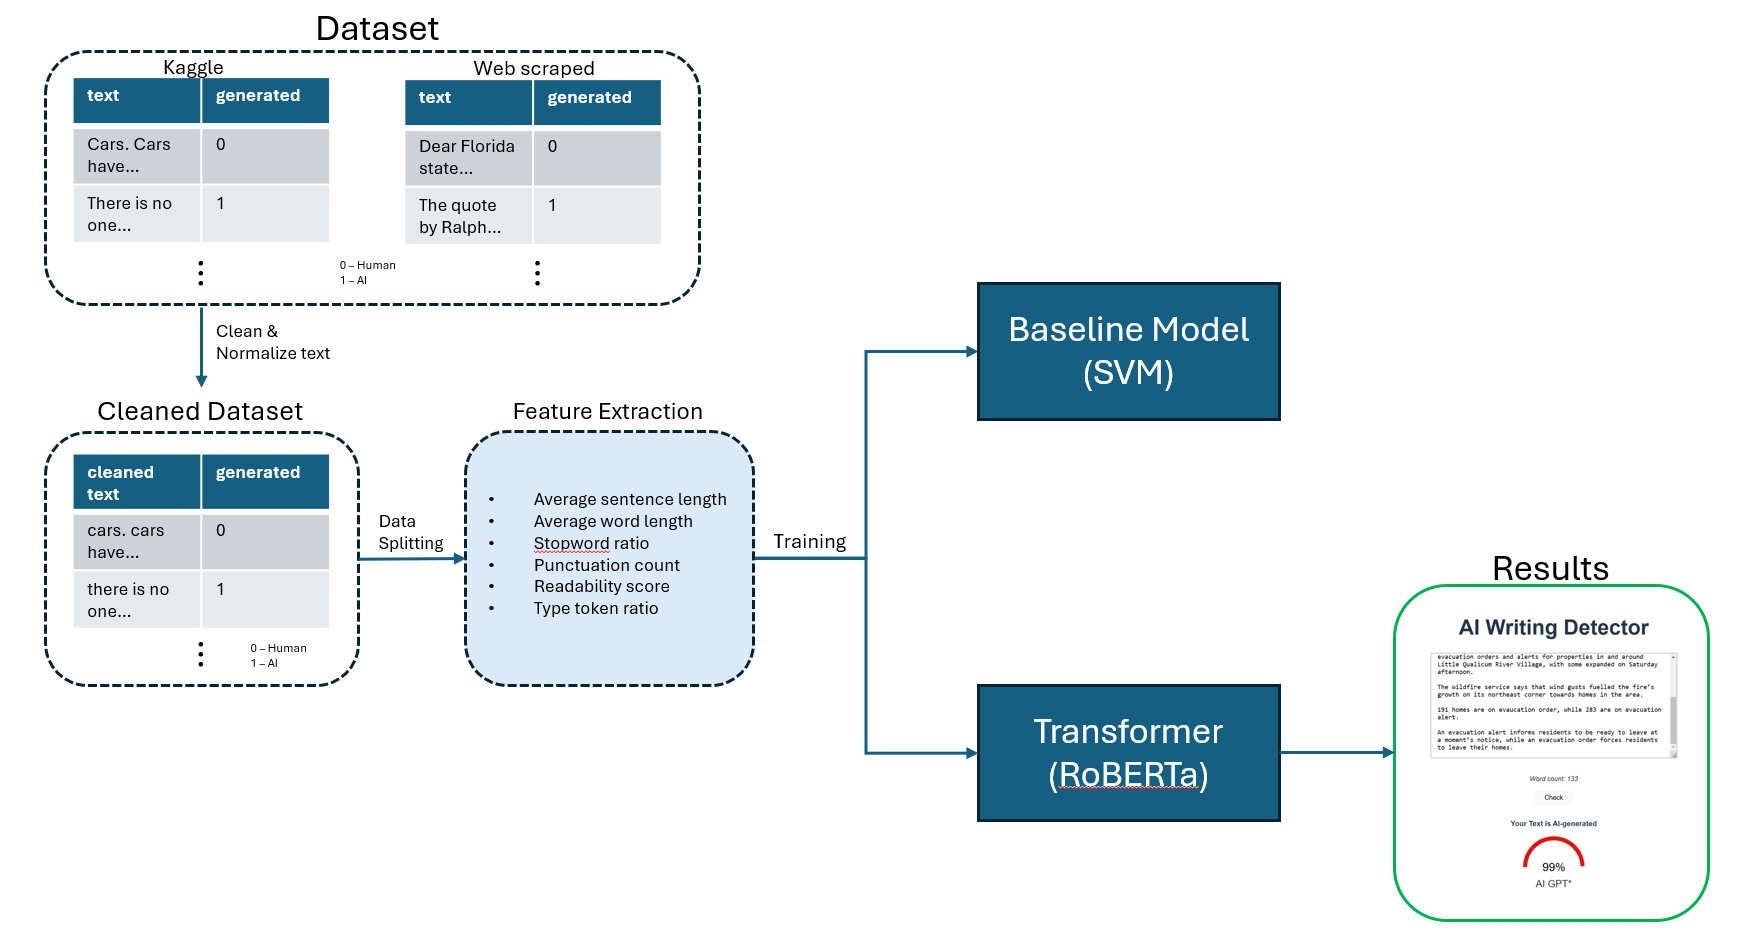
\includegraphics[width=0.9\linewidth]{illustrationFinal.png}
    \caption{Illustration of Overall Model} 
    \label{fig:pipeline}
\end{figure}

\section{Background \& Related Work}

\subsection{Related Papers}

\textbf{``Detecting Generative Artificial Intelligence Essays using Large Language Models: Machine and Deep Learning Approaches''}  ~\citep{Approaches}

This study analyses the efficacy of different deep learning models to identify human written and AI written essays. The algorithms it discusses are logistic regression, Support Vector Machine (SVM), decision trees, random forests, K-Nearest Neighbours (KNN), and Long Short Term Memory (LSTM). The research used Term Frequency-Inverse Document Frequency (TF-IDF) to prepare their data. It found that SVM and LSTM were the most accurate algorithms, though LSTM is more demanding computationally.

\textbf{``Deep learning detection method for large language models-generated scientific content''} ~\citep{DeepLearning2024}

This paper outlines a model called AI-Catcher developed to identify AI generated writing, citations, and data in scientific papers, treated as a binary classification problem. AI-Catcher uses two models to identify human versus AI generated text: the MLP and a Convolutional Neural Network (CNN). For the MLP, it prepares the data through text cleaning, text encoding, and padding. The MLP model then has five hidden layers, each with 256 neurons, where each layer applies a linear transformation and then ReLU activation. For the CNN model, it prepares the data through extraction of thirteen linguistic and statistical features from the text. Then, it uses the embedding layer to put the encoded integers into vectors, followed by a dropout layer, and then a convolutional layer connected to a global max pooling layer. The results of the two are then concatenated into a single feature vector, which goes through two additional hidden layers. The accuracy, precision, recall, and F1 score of the model were assessed based on confusion matrices. This research was only conducted using scientific papers written by humans or generated by ChatGPT (as opposed to other LLMs).

\textbf{``Detecting AI-generated essays: the ChatGPT challenge''} ~\citep{AIessays2023}

This research paper from early 2023 investigates effective algorithms to identify human and ChatGPT generated essays. They used a n-gram bag-of-words (BOW) language model for the classifier input with n=5. They tested the performance of Support Vector Machine, Naïve Bayes, Logistic Regression, Random Forest, and Neural Network classification algorithms and then tested the performance of an Ensemble Learning (EL) classifier with the five algorithms fed to it. The findings stated that their SVM, which was modified to eliminate False Negatives entirely, was the most efficient algorithm. The study emphasized eliminating False Negatives (human written essays labelled as AI) due to the ethical implications of incorrectly blaming students for plagiarism with ChatGPT. SVM alone had a slightly lower accuracy than EL, but had better recall and F2 scores. Their SVM model also had fewer False Negatives than OpenAI Detector, GPTZero, and Copyleaks on test data and a 100\% accuracy in detecting human-written essays, despite a lower overall accuracy. This research did also have a relatively small sample size, with 230 total essays for training and 150 for testing (Cingillioglu, 2023).

\subsection{Current Software Solutions}

\textbf{GPTZero} ~\citep{GPTZero}

GPTZero is an AI detector that scans for AI generated writing on a sentence, paragraph, and document level. It can detect AI written content generated by ChatGPT, GPT-4, GPT-3, GPT-2, LLaMA, and derivatives of those models. It claims to have a 99\% accuracy and has an extension that can be added to Google Classroom and Google Docs. It can also identify if a text is entirely human written, entirely AI written, or mixed. However some of its features are locked behind a paid subscription, such as its ability to indicate the most human or AI written parts of a sample of writing and the number of characters, words, or files that can be submitted to it at a time, and it is also primarily for the analysis of English text.

\textbf{Copyleaks} \citep{Copyleaks}

Copyleaks is a plagiarism detector and AI detector. It works with 30+ languages and claims to have a 99.8\% accuracy and a 0.2\% false positive rate. It can detect text written by LLMs like ChatGPT, Gemini, DeepSeek, Claude, Jasper 3, LLaMA, and T5. It also shows the percentage of AI in a piece of text and can account for different detection sensitivity levels. It claims to have the capability to identify plagiarism and paraphrasing done with AI and that it can identify human written, AI written, and mixed text. It has a minimum requirement for the number of characters (350) to accurately determine the presence of AI. Copyleaks also has Google Docs extension and mostly requires a paid subscription, with only a limited number of free uses.

\textbf{Grammarly} ~\citep{Grammarly}

Grammarly, an AI based grammar checker, also has its own AI detector. It can detect writing generated by Grammarly, ChatGPT, Google Gemini, and Claude, and it can show the percentage of text that is AI generated. However, it is only available with certain paid subscriptions and they have not stated the accuracy rate of their checker.

\section{Data Processing}
We used a publicly available dataset from Kaggle consisting of approximately 500,000 English text samples labeled either as human-written (generated = 0) or AI-generated (generated = 1). To further diversify and expand our dataset, we web scraped a few texts from four different websites using Selenium and BeautifulSoup. Table 1 shows a few examples from the combined dataset. 

\begin{table}[H]
\caption{Table 1: Snippet of the CSV dataset}

\begin{flushleft}
\href{https://www.kaggle.com/datasets/shanegerami/ai-vs-human-text}{\texttt{https://www.kaggle.com/datasets/shanegerami/ai-vs-human-text}}\\
Zahra Web1\\
Zahra Web2\\
Zahra Web3\\
Zahra Web4
\end{flushleft}

\vspace{0.5em}

\begin{tabular}{|p{10cm}|c|}
\hline
\textbf{text} & \textbf{generated} \\
\hline
Join the seagoing cowboys today! Wave an irreplaceable experience\ldots & 0 \\
\hline
The rise of electric cars has been one of the most important developments\ldots & 1 \\
\hline
\end{tabular}
\end{table}

To prepare the data for training, we passed each text sample through a filtering pipeline to ensure consistency across all data. For each text, the following cleanings were performed:
\begin{itemize}
    \item \textbf{Contraction Expansion:} All contractions were expanded to their full forms (e.g., ``can't'' to ``cannot'') using Python's \texttt{contractions} library.

    \item \textbf{Punctuation and Symbols:} Non-alphanumeric symbols were removed while retaining essential punctuation marks to preserve stylistic information (e.g., ",.?!;:()).

    \item \textbf{Case Normalization and Whitespace Removal:} All text was converted to lowercase and extra whitespace (e.g., multiple newlines) was removed to ensure uniform formatting.

    \item \textbf{Text Length Filtering:} Samples with fewer than 350 words or fewer than two complete sentences (identified using \texttt{nltk.sent\_tokenize}) were removed to ensure sufficient content for meaningful analysis.

    \item \textbf{Near-Duplication Removal:} We employed MinHash-based Locality Sensitive Hashing (LSH) via the \texttt{datasketch} library to remove near-duplicate entries. This step mitigates redundancy, particularly common in AI-generated texts that often follow templated structures.
\end{itemize}

Table 2 presents a side-by-side comparison of raw and cleaned text samples. Since the cleaning process filters out shorter texts and only retains ones with at least 350 words, we have only included a short sample here for illustration purposes, which includes contraction expansion and case normalization. 

\begin{table}[H]
\caption{Table 2: Snippet the Raw vs Cleaned Human-Written Text}
\begin{tabular}{|p{6.5cm}|p{6.5cm}|}
\hline
\textbf{Raw Text} & \textbf{Cleaned Text} \\
\hline
Lastly, the electoral college is irrational like seriously what idiotic person came up with this. I will say this again, but a monkey could of made a better system than this. ``Under the electoral college system, voters vote not for the president, but for a slate of electors, who in turn elect the president........Who are the electors? They can be anyone not holding public office. Who picks the electors in the first place? It depends on the state. Sometimes state conventions, sometimes the state party's central committee, soemtimes the presidential candidate themselves. Can voters control whom their electors vote for? Not always. DO voters sometimes get confused about the electors and vote for the wrong candiate? Sometimes" Plumer, Source 2 I know this statement says it all because how could one simply not want popular vote after reading this. & lastly, the electoral college is irrational like seriously what idiotic person came up with this. i will say this again, but a monkey could of made a better system than this. ``under the electoral college system, voters vote not for the president, but for a slate of electors, who in turn elect the president........who are the electors? they can be anyone not holding public office. who picks the electors in the first place? it depends on the state. sometimes state conventions, sometimes the state party's central committee, soemtimes the presidential candidate themselves. can voters control whom their electors vote for? not always. do voters sometimes get confused about the electors and vote for the wrong candiate? sometimes" plumer, source 2 i know this statement says it all because how could one simply not want popular vote after reading this.  \\
\hline
\end{tabular}
\end{table}

After the cleaning process, a total of 126163 text samples remain, with a total of 80742 samples for human-written and 45421 samples for AI-generated. We decided to keep all the cleaned data to maximize training volume and generalization. To address this imbalanced dataset, we plan to evaluate performance using balanced metrics such as F1-score, precision, recall, and accuracy for each class.  


\section{Architecture}
\begin{figure}[htbp]
    \centering
    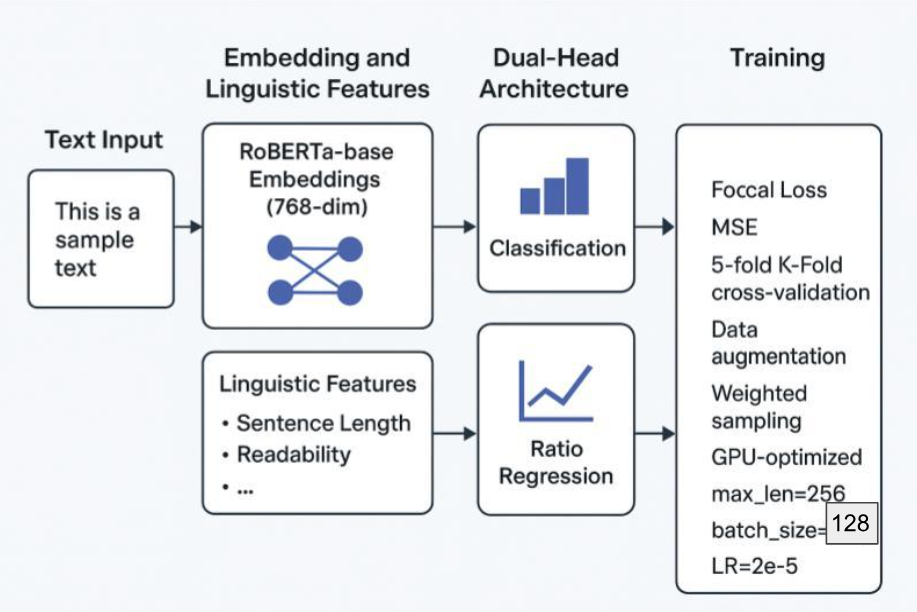
\includegraphics[width=0.9\linewidth]{architecture.png}
    \caption{RoBERTa Model} 
    \label{fig:pipeline}
\end{figure}
To ensure a robust and diverse dataset, we will undertake an extensive data collection and processing effort, prioritizing originality and rigor over the use of pre-existing datasets. Our data is sourced from multiple origins to enhance generalization:This hybrid neural model addresses the growing challenge of distinguishing human-written, AI-generated, and mixed-origin text through a sophisticated dual-task architecture. The system simultaneously classifies text origin (human/AI/mixed) and predicts precise AI-to-human ratios in mixed-content samples, providing both categorical and continuous metrics for analysis. At its foundation lies RoBERTa-base, which generates 768-dimensional semantic embeddings through its transformer architecture, offering deep contextual understanding of text. These embeddings are enhanced with 10 carefully selected linguistic features capturing stylistic patterns - including average sentence length, lexical diversity (type-token ratio), readability scores (Flesch reading ease), and phonological characteristics (syllable distribution). The linguistic features undergo dimensionality reduction through a dedicated 64-unit layer before being concatenated with RoBERTa's output, creating a rich 832-dimensional combined representation.\\

The model's innovative dual-head architecture processes this fused representation through parallel pathways. A classification head with two hidden layers (128~$\rightarrow$~64 units) employing ReLU activation and dropout ($p = 0.2$) handles the three-way text categorization, while a regression branch with 32-unit hidden layers predicts mixture ratios using sigmoid activation. Training employs Focal Loss ($\gamma = 2$) for the classification task to handle class imbalance and Mean Squared Error for ratio prediction, with a combined loss function weighted to balance both objectives. The implementation demonstrates strong computational efficiency, operating with a maximum sequence length of 256 tokens (optimized from RoBERTa's standard 512), batch size of 32, and learning rate of $2 \times 10^{-5}$ when trained on GPU hardware.\\

Robust training protocols ensure model reliability, including 5-fold K-Fold cross-validation with stratified sampling and early stopping (patience=2) to prevent overfitting. These techniques contribute to the model's consistent ~80\% classification accuracy across validation folds while maintaining precise ratio estimation capabilities (MSE ~0.15). 


\section{Baseline Model}








\section{Quantitative Results}
For training our model, we used the cross-entropy loss function and had a mini-batching size of 128 as well as trained our model on 4 epochs. 
Due to limited GPU memory and a large dataset, we used the cross-entropy loss function for its ability to assign higher gradients to wrong predictions, enabling the model to learn faster. We also used mini-batching with batches of 128 samples to speed up training by computing gradients more efficiently. However, this has caused  some noise in the training and validation curves due to differences in complexity and gradients between the batches. As seen in Figure xx, the model converges around ~78\%, which is the final training accuracy with some oscillations between ~70\% to ~90\%. With no large divergences, the model is relatively stable. The validation curve also steadily increases along the training accuracy curve and reaches a final score of ~81\%, indicating that our model is not overfitting and generalizing well. Our model is accurately predicting human and AI samples around ~78\% of the time and based on the curves and with limited GPU memory, the model is performing well.

\begin{figure}[htbp]
    \centering
    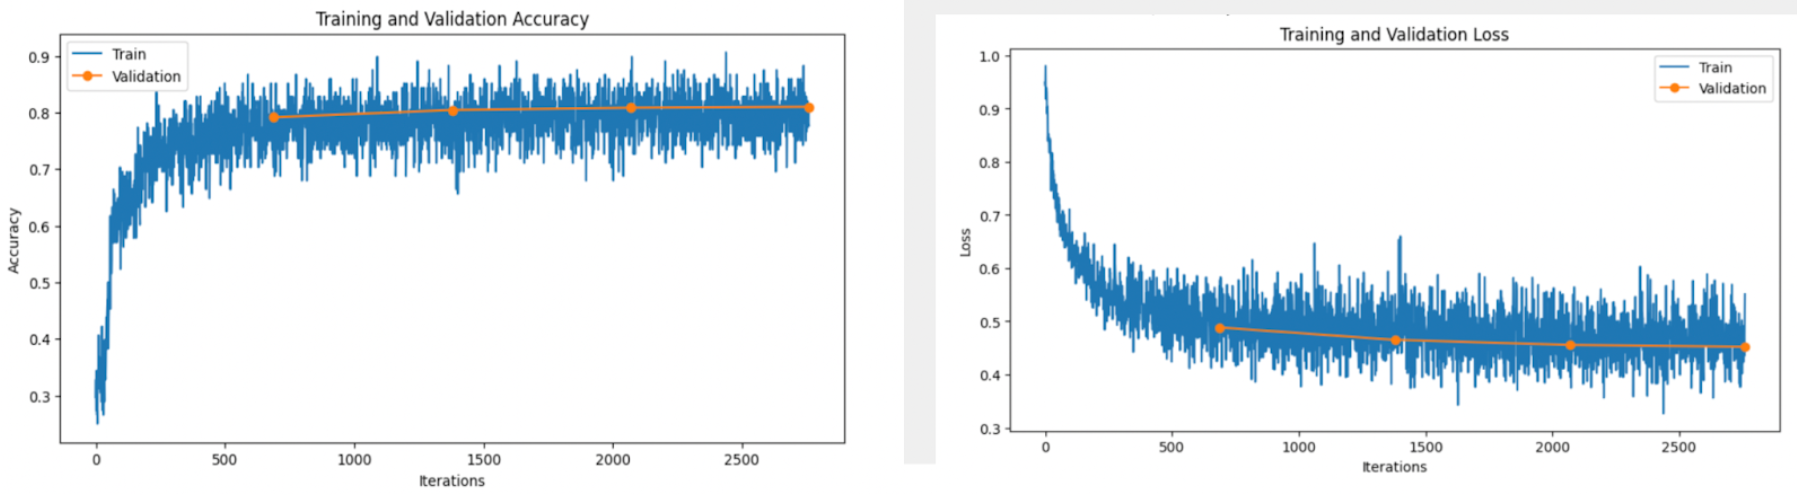
\includegraphics[width=0.9\linewidth]{trainValcurve.png}
    \caption{Training and Validation Curves for Accuracy and Loss Respectively} 
    \label{fig:pipeline}
\end{figure}




\section{Qualitative Results}
For qualitative results, we evaluated the model on 12000 human samples and 6800 AI samples, each containing at least 350 words to ensure that there is enough text for detection. Figure xx is a classification report for both classes to better understand model performance.

\begin{figure}[htbp]
    \centering
    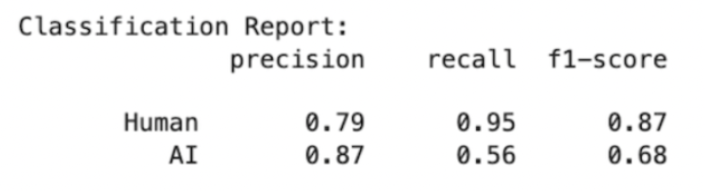
\includegraphics[width=0.9\linewidth]{classReport.png}
    \caption{Classification Report for AI and Human Samples} 
    \label{fig:pipeline}
\end{figure}

We measured the precision (how often predicted positives are correct), recall (how many correct positives actually found in total data), and F1 score(balance between precision and recall scores). From this, we observe that the model has a strong F1 score of ~87\% for Human sample detection, which is the combination of the strong recall score for Human samples. The model predicted ~95\% of the Human samples in the whole dataset correctly and has an accuracy of being ~79\% correct from all of the Human predictions. However, the model has misclassified AI samples as Human often, shown in the recall score of ~56\%. An example of the model predicting an AI sample wrong is shown in Table 3.

\begin{table}[H]
\centering
\caption{Human and AI samples for Model Predictions vs True Labels examples}
\begin{tabular}{|c|c|c|}
\hline
\textbf{Sample} & \textbf{Model Prediction} & \textbf{True Label} \\
\hline
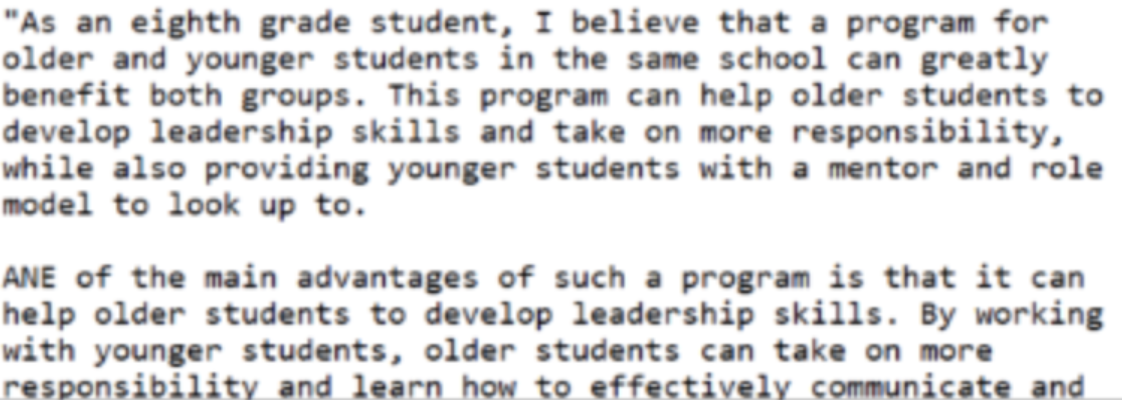
\includegraphics[width=5cm]{sample1.png} & Human & AI \\
\hline
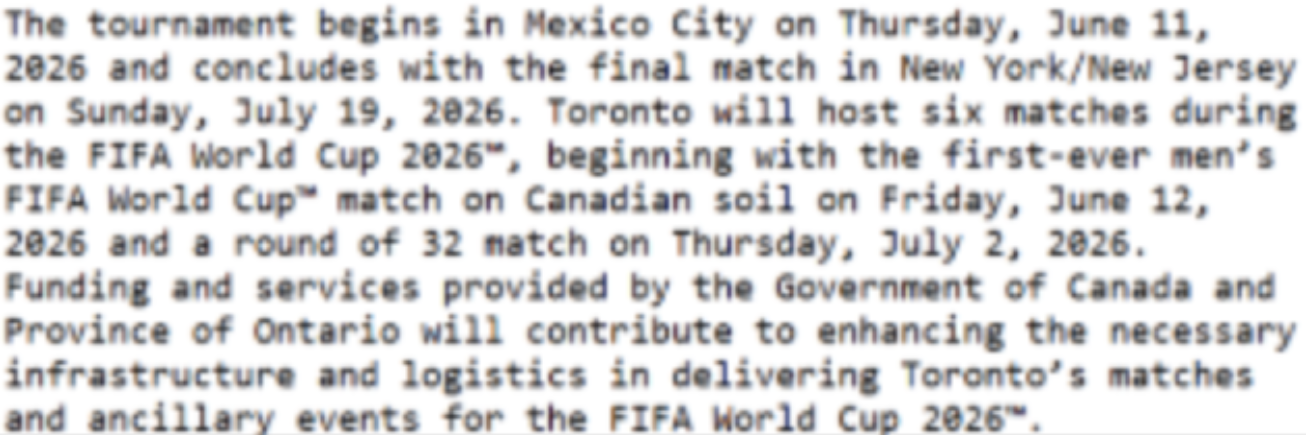
\includegraphics[width=5cm]{sample2.png} & Human & Human \\
\hline
\end{tabular}
\end{table}

From the sample examples, the model was able to correctly identify the human sample, but just like the samples above, a lot of the AI samples have been mislabeled as human. The model predicting human-generated over AI-generated more often may be due to the imbalance in training data, where we were able to attain more human samples over AI samples. However, the AI precision score exceeds the human precision score, showing that the model predicts the AI samples carefully but mostly correctly. With all the human and AI precision and recall scores, the model has an overall average of being ~81\% accurate in labeling the whole dataset, similar to the value we got in quantitative results. With these results, we need to focus more on improving the AI classification score, which should increase our overall model accuracy.


\section{Evaluate Model on New Data}
To ensure our model genuinely understands text patterns rather than memorizing training examples, we implemented a rigorous evaluation process using completely unseen data. The model was tested on fresh human-written and AI-generated texts that were never exposed during training or validation, processed through the exact same preprocessing pipeline used in development. This includes identical tokenization, linguistic feature extraction, and normalization steps to guarantee fair assessment conditions. We measure performance not just through basic accuracy, but with comprehensive metrics including precision, recall, and F1 scores for all classification categories (Human and AI), plus mean squared error for the ratio prediction task.

The evaluation results demonstrate strong generalization capabilities, with the model maintaining approximately 80\% accuracy on novel text samples. This consistent performance across different test batches confirms it learned meaningful patterns rather than overfitting to training data. The ratio predictions show logical gradients, with smooth confidence transitions between purely human and purely AI texts, and errors primarily occurring in genuinely ambiguous cases like highly formal human writing. Our testing approach completely isolates the evaluation environment - loading only pretrained weights and using separate test data files to prevent any accidental data leakage. The model processes raw, unmodified text inputs under the same conditions it would face in real-world deployment, handling varied text lengths and complexities while maintaining its sequence length constraints and batch processing parameters.

However, the model demonstrates a noticeable bias toward classifying text as human-written rather than AI-generated, evidenced by its performance metrics on the test set. While it achieves excellent recall for human text (95\%)—correctly identifying nearly all genuine human writing—its precision (79\%) reveals frequent false positives where AI content is mistakenly labeled as human. Conversely, the model shows higher precision (87\%) but lower recall (56\%) for AI detection, meaning that when it does identify text as AI-generated, it’s usually correct, but it misses nearly half of actual AI content by erroneously categorizing it as human. This imbalance likely stems from the training data composition—with fewer AI examples available, the model becomes overly cautious about assigning the AI label, defaulting to ``human" in ambiguous cases. The 81\% overall accuracy, while strong, masks this asymmetry in detection capability.

\section{Discussion}



\section{Ethical Considerations}
AI detection tools have ethical issues such as bias and accuracy. A false positive can be detrimental to an individual’s career as this is tied to their credibility. Bias can put certain groups at higher risk of receiving a false positive such as non-native English speakers. They are more prone to receiving a false positive compared to native speakers due to differences in writing styles and levels of sophistication (Myers, 2023). Additionally, the risk of a biased model is that individuals begin to fear being flagged, even without AI usage, limiting creativity. As writing is a creative form of expression, detecting different styles is challenging, putting individuals at risk even without any AI usage.
To limit this problem and prevent our model from becoming biased or overfitting to a certain writing style, our model is trained on a large dataset of both human and AI samples. This way, our model has a lot of samples to learn from, being able to detect a variety of writing patterns, lowering the risk of a false positive. 


\section{Project Difficulty/Quality}
Distinguishing between AI-generated and human-written text is not an easy task because large language models are designed to generate content that is fluent, grammatically correct, and stylistically similar to human writing. Newer, more advanced LLMs are more powerful and better at generating even more fluent language, making current detection tools less effective. Unlike other binary classification tasks where two classes have clear and distinct patterns, such as spam and non-spam messages, the differences in AI and Human texts are more subtle. To better mimic the real-world scenarios, we normalized the dataset during preprocessing by lowercasing all texts, removing any extra spacings, and performing deduplication to ensure that the model generalizes better across a wide range of texts. To address this challenge, we designed a hybrid model that combines RoBERTa-based contextual embeddings with linguistic features such as sentence length, stopword ratio, and readability score, to capture both surface-level stylistic differences as well as deep semantic meanings. Despite the difficulty of the problem, our model achieved 81\% test accuracy. 


\hypersetup{
    colorlinks=true,
    linkcolor=blue,
    urlcolor=blue
}

\section{Link to Github/Colab}
\noindent
\href{https://github.com/shill7/APS360_Project}{\underline{\textcolor{blue}{GitHub Repository}}}

\label{last_page}

\bibliography{APS360_ref}
\bibliographystyle{iclr2022_conference}

\end{document}